\documentclass[a4paper,10pt]{article}
\usepackage[utf8]{inputenc}
\usepackage{geometry} %自定义布局
\usepackage{multicol} %双栏
\usepackage{graphicx} %图像
\usepackage{amsmath} % 数学单位等等
\usepackage[runin]{abstract} %摘要修改 摘要标题添加到摘要正文段前
\usepackage{booktabs}%三线格
\usepackage{float}%浮点
\usepackage{cite}%引用
\usepackage{pdfpages}%pdf合并
\usepackage{caption}
\usepackage{graphicx, subfig}
\usepackage[colorlinks,
            linkcolor=blue,       %%修改此处为你想要的颜色
            anchorcolor=blue,  %%修改此处为你想要的颜色
            citecolor=blue,        %%修改此处为你想要的颜色,例如修改blue为red
            ]{hyperref}
\usepackage{appendix}
\geometry{a4paper,left=1.6cm,right=1.6cm,top=2cm,bottom=2cm}
\graphicspath{{picture/},{pics/}}
%opening
\title{}
%%%标题加粗
\author{Kangyao Ma, Mingbai Zeng, Yimeng Yuan, Haozhan Yuan}
\date{}


\begin{document}


\includepdfmerge{first.pdf}


\maketitle


\setlength{\absleftindent}{0pt}
\setlength{\absrightindent}{0pt}
\setlength{\abstitleskip}{-1.5em}
\abslabeldelim{:}
\renewcommand{\abstractnamefont}{\itshape\bfseries}
\renewcommand{\absnamepos}{flushleft}
\begin{abstract}
\textit{\small Reverse genetics was applied in this laboratory practical to investigate the function of the gene ANID\_08549 in Aspergillus nidulans. A knockout cassette was constructed consisting of upstream and downstream homologous fragments of the target gene and selective gene Af-$pyrG^+$ for specifically deleting the target gene and inserting a selective gene for the mutant screening. The target gene is expected to be deleted by homologous recombination and the selective gene is inserted to replace it. After screening by inoculation on the selective agar and the PCR verification, it was confirmed that the mutant had been obtained in this experiment. To complete perform reverse genetics, further experiment is required for phenotype screening and function determination of the target gene. Suggestions to enhance the accuracy of the experiments included increasing primer specificity, adjusting annealing temperature and sample picking technique. }
\end{abstract}


\hrule


\begin{multicols}{2}
\section{Introduction}


Driven by the advances in modern biotechnology, the development of genomics has provided us with a new perspective on understanding gene function, especially through reverse genetics. Reverse genetics provides a novel methodology for investigating gene function by analyzing the phenotypic consequences after modification of the target gene\cite{hardy2010reverse}.Two main approaches of reverse genetics which focus on genome alternation are one applied random mutagenesis by chemical or insertion and the other by the alternation of the target gene specifically by homologous recombination\cite{hardy2010reverse}.

%\noindent %无缩进
This experiment aims to explore the function of gene ANID\_08549 in Aspergillus nidulans which is a fungi model organism that has been extensively studied\cite{son2023regulators}. In order to apply the deletion of the gene ANID\_08549 and for the efficient screening of the mutant, a knockout cassette was constructed in this experiment. Knockout cassette is a fragmented DNA which consists of upstream and downstream homologous fragments of the target gene for the gene deletion by the homologous recombination and a selective gene for the mutant screening\cite{xiaoli2015efficient}.The knockout cassette of this experiment was constructed by amplification and ligation of the homologous arms of the gene ANID\_08549 and selective gene Af-$pyrG^+$. The Af-$pyrG^+$ gene which encodes orotidine 5'-phosphate decarboxylase was derived from the Aspergillus fumigates which is an animal pathogen\cite{d1996selection}\cite{wassano2020aspergillus}.The gene ANID\_08549 will be deleted specifically by the knockout cassette by the homologous recombination and the Af-$pyrG^+$ gene will be inserted in replacing the target gene.

The A. nidulans pyrG89 strain was used in this experiment. The strain has a mutation in a gene nkuA, which encodes Ku70 which is required for non-homologous recombination and in gene pyroA4 which encodes pyridoxine which acts as a coenzyme of the orotidine 5'-phosphate decarboxylase to synthesis uridine monophosphate (UMP) and subsequently produce uridine and uracil\cite{yee2022investigating}. The origin pyrG89 strain could not survive at the agar without uridine and uracil even adding the pyridoxine\cite{nayak2006versatile}. Only if the strain that has been successfully transformed and inserted the orotidine 5'-phosphate decarboxylase encoded by Af-$pyrG^+$ gene into the genome by homologous recombination can survive at the selective agar plate in which the absence of the uridine and uracil and added the pyridoxine.


\section{Material and Method}





\subsection{PCR amplification of knockout cassette DNAs }
After amplification of the cassette DNA, the amplified product underwent verification by extracting 1 \textmu L and transferring it to 9 \textmu L of diluted loading buffer, followed by thorough mixing. Subsequently, all samples were loaded onto an agarose gel. A 5 \textmu L DNA ladder was added to the spare channel of the electrophoresis tank, after which the tank's cover was replaced, and the gel was electrophoresed at 75 volts for one hour. Finally, a UV transilluminator was used to visualize and confirm the presence of the deletion cassette.


\subsection{Aspergillus transformation}
The A. nidulans strain pyrG89 $\Delta$nkuA pyrA4 was cultured overnight in liquid media. Following this, the mycelia were harvested and subjected to a two-hour incubation in an isotonic solution containing a cell-wall-degrading enzyme to remove the cell wall, resulting in the formation of protoplasts. The protoplasts were subsequently filtered, centrifuged, and washed before being suspended in a transformation solution containing $CaCl_2$, which facilitated the uptake of DNA into the cells.


\subsection{Transformation of Aspergillus with knockout cassette DNAs}

To initiate the transformation process, two 50 mL plastic tubes with sterile screw caps were placed on ice. One tube was labeled "ANID\_08549," and the second tube was labeled as the negative DNA control. 100\textmu L of protoplasting solution was gently pipetted into both tubes. Subsequently, 20 \textmu L of DNA was added to the ANID\_08549 tube, and 20\textmu L of transformation solution was added to the negative control tube. Using a tip with the end cut off, 50\textmu L of PEG solution was transferred to each tube, with care taken to move the tip slowly up and down to ensure accurate volume addition without any solution lost to the tube walls. The tubes were gently rolled and then incubated on ice for 20 minutes.Following this, 1 mL of PEG was added to each tube, and the mixture was shaken and left on the bench for an additional 5 minutes as a mild heat shock treatment. Subsequently, 5mL of transformation solution was added to each tube, and they were returned to ice. The plates were properly labeled, and approximately 15mL of molten medium was poured into each plate, ensuring that the agar filled only about 80\% of the tubes before covering them with lids. The tubes were then slowly turned two or three times to facilitate gentle mixing, followed by final incubation for one week.


\begin{center}
{\footnotesize Table 1. Materials needed for this experiment}
\begin{table}[H]
\footnotesize
\begin{tabular}{lc}
\toprule [1pt]
\textbf{PCR amplification of knockout}&\textbf{Explanation}\\
\textbf{cassette DNAs}& \\
\hline
Microcentrifuge tube&\\
PCR amplification knockout box&20\textmu L/tube\\
Load buffer&\\
DNA ladder&5 \textmu L\\
A. nidulans strain pyrG89 pyrA4 $\Delta$nkuA&\\
Isotonic solution &\\
\hline
\textbf{Transformation of Aspergillus with }&\\
\textbf{knockout cassette DNAs}&\\
\hline
$5\times10^7$/mL protoplast &200\textmu L\\
DNA&20\textmu L\\
Transformation solution($CaCl_2$)&10mL \\
50\% PEG&2 mL \\
Molten regeneration media&50mL\\
50 mL sterile plastic tubes&2\\
Agar plates with regeneration media&6\\
\hline
\textbf{DNA extraction}&\\
\hline
Fungal cells&\\
Buffer FG1&1800\textmu L\\
Buffer FG2&520\textmu L\\
Buffer FG3&0.9mL\\
RNase&15\textmu L\\
Absolute &2.7mL\\
DNA Wash Bufferv & 1.8mL \\
Elution Buffer & 300\textmu L\\
1.5 mL tube & 6\\
DNA Mini Column&3\\
2 mL Collection Tube&4\\
\hline
\textbf{PCR}&\\
\hline
10X dNTP mix&16\textmu L\\
5X Q-solution&32\textmu L\\
$ddH_2O$&65.6\textmu L\\
Taq polymerase&8\textmu L\\
DNA or $H_2O$ for control&32\textmu L\\
An-For&3.2\textmu L\\
AN-Rev&1.6\textmu L\\
Af-pyrG-Rev&1.6\textmu L\\
\hline
Gel electrophoresis&\\
\hline
1\% agarose in 1X TAE&100mL\\
5\% polyacrylamide in 5X TBE&\\
6X Loading buffer &5 \textmu L\\
Molecular maker &N3231S\\
\bottomrule [1.5pt]
\end{tabular}
\end{table}
\end{center}


\subsection{Amplification of transformants}
After one week of incubation, the transformation plates were examined, and the number of colonies was counted. Subsequently, three potential transformants were selected using sterile needles. Each transformant was inoculated onto an individual agar plate, which was then securely sealed with tape and labeled with the date and group 24. The plates were placed in an incubator for another week for cultivation.


\subsection{DNA extraction}
Two potential transformants were selected and transferred, along with their mycelia and conidia, using a small spatula to two labeled 1.5 mL tubes containing 600\textmu L of FG1 buffer. The tubes were then shaken vigorously by vortex for one minute. Additionally, one original untransformed colony was selected for the same treatment. Subsequently, 5\textmu L of RNase was added to each tube, and the tubes were incubated at 65\textcelsius\ for ten minutes in a heat block. All samples were manually inverted twice during the incubation period. After incubation, 140\textmu L of buffer FG2 was added to each tube, and the tubes were vortexed to mix. The tubes were then placed on ice for 5 minutes before being centrifuged at 10,000 xg for 10 minutes. The resulting supernatants were transferred to new 2 mL tubes, with each tube containing 600\textmu L of supernatant. Subsequently, 300\textmu L of buffer FG3 was added to all tubes, followed by the addition of 900\textmu L of absolute ethanol. The samples were thoroughly mixed and applied to the corresponding DNA minicolumns. The minicolumns were centrifuged at 10,000 xg for 1 minute, and the flow-through liquid was discarded. After adding 600\textmu L of DNA wash buffer to each column, the columns were centrifuged again at 10,000 xg for 1 minute, and the flow-through liquid was discarded. The washing steps were repeated twice, followed by another centrifugation for 2 minutes at 10,000 xg. Subsequently, 100\textmu L of preheated elution buffer at 70\textcelsius\ was transferred to each minicolumn, and the tubes were incubated at room temperature for 4 minutes. Finally, all DNA samples were centrifuged once more at 10,000 xg for one minute to obtain eluted DNA, which was then available for PCR analysis.


\subsection{PCR amplification of deletion mutants}
For setting up the PCR experiment, all tubes were labeled accordingly. Each tube was then added 0.8\textmu L of mixed primer sets and 4\textmu L of the corresponding DNA. Other components, including 8.2\textmu L of $H_2O$, 2\textmu L of dNTP mix (10X), 4\textmu L of 5X Q-Buffer, and 1 \textmu L of Taq DNA polymerase, were also included in the PCR tubes. For the water control group, the DNA solution was substituted with the same volume of distilled water. The tubes were then ready for the PCR process.


\subsection{Gel electrophoresis}
To prepare a 1\% agarose gel in 1X TAE, 1g of agarose was weighed using an electronic scale. The agarose was then added to 100 mL of 1X TAE in a flask. The flask was microwaved with a loose lid to fully dissolve the agarose. Once the agarose solution cooled to around 60°C, 10\textmu L of Gel Red (1:10,000) was added and mixed gently. The melted gel solution was poured into a gel stand, with both ends taped, and a comb was placed to create wells. After waiting for 30 minutes for the gel to solidify, the masking tapes at the tray ends were removed. The tray, along with the gel, was then placed into an electrophoresis tank. 1X TAE was added to the tank until the gel surface was fully submerged, and then the comb was carefully removed.Next, 5\textmu L of loading buffer (6X) was added to each sample, and 10\textmu L of molecular marker was loaded onto the gel. Finally, the gel electrophoresis was run for 45 minutes at 75 volts.


\iffalse
\begin{center}
{\footnotesize Table 2. Outline of the mutagenesis for each plate}
\vspace{0pt}
\begin{table}[H]
\footnotesize
\begin{tabular}{ccccc}
\toprule [1.5pt]
Plate Number&Cell dilution to be plated&Plate type&Tryptophan concentration(\textmu g/mL)&Treatment\\
\hline
1&$10^0$&SA3&0&$Trp^+$ strain and $Trp^-$ strain\\
2&$10^0$&SA3&0&None\\
3&$10^0$&SA2&1&None\\
4&$10^0$&SA1&0.25&None\\
5&$10^{-5}$&NA&Non-limiting&None\\
6&$10^{-6}$&NA&Non-limiting&None\\
7&$10^0$&SA2&1&Spot test with 1\% MMS\\
8&$10^0$&SA2&1&Spot test with 1\% MMS\\
9&$10^0$&SA2&1&Spot test control (water)\\
10&$10^0$&SA1&0.25&Treat with 1\% MMS then plate\\
11&$10^0$&SA2&1&Irradiate with UV light for 20 sec\\
12&$10^0$&SA2&1&Irradiate with UV light for 40 sec\\
\bottomrule [1.5pt]
\end{tabular}
\end{table}
\end{center}
\fi


%\begin{figure}[htbp]
%\centering
%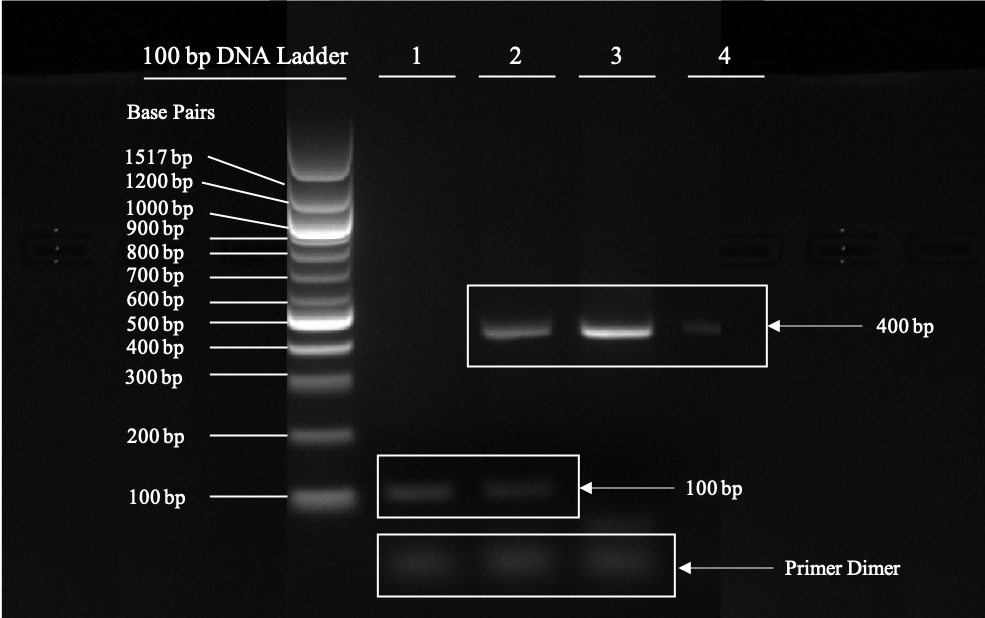
\includegraphics{tpa25.png}
%\caption{bionux}
%\end{figure}


\section{Results and Analysis}


%The pyrG89 strain which has was used in this experiment. The strain has a mutation in a gene nkuA, which encodes Ku70 which is required for non-homologous recombination and in gene pyroA4 which encodes pyridoxine which acts as a coenzyme of the orotidine 5'-phosphate decarboxylase to synthesis uridine monophosphate (UMP) and subsequently produce uridine and uracil. The origin pyrG89 strain could not survive at the agar without uridine and uracil even adding the pyridoxine. Only if the strain that has been successfully transformed and inserted the orotidine 5'-phosphate decarboxylase encoded Af-$pyrG^+$ gene into the genome by homologous recombination can survive at the selective agar plate in which the absence of the uridine and uracil and added the pyridoxine.

%%%
%\begin{center}
%{\footnotesize Table 3. Count of bacterial colonies on each plate}
%\vspace{0pt}
%\begin{table}[H]
%\setlength{\tabcolsep}{5pt}
%\footnotesize
%\begin{tabular}{ccccccccccccc}
%\toprule [1pt]
%Plates&1&2&3&4&5&6&7&8&9&10&11&12\\
%\hline
%colonies&/&0&2&16&4&0&32&59&5&2&7&3\\
%\bottomrule [1pt]
%\end{tabular}
%\end{table}
%\end{center}
%%%


The uridine and uracil absence and pyridoxine adding agar plates were used to screen out the transformants. As Figure\ref{fig1} shows, after one week of incubation, the putative transformants which had been inoculated on the selective agar plates Test 1 and 4 had grown and generated 5 large colonies with a dark green colour. At around and above the surface of colonies, there have generated large amounts of white colour hyphae. The control plates did not generate any colony which followed the expectation that the strains that were not treated with transformation and not possessing the Af-$pyrG^+$ gene would not survive at the agar plates with the absence of uridine and uracil. Tests 2 and 3 have generated two colonies but the size of the colonies is small and the morphology of the colonies is distinct to the colonies generated by Tests 1 and 4. The colony which Test 3 generated had a large proportion of hyphae while the colony that Test 2 generated had less proportion of hyphae. Due to the significant differences in morphology, these two colonies are not identified as putative transformants.


\begin{figure}[H]
\centering
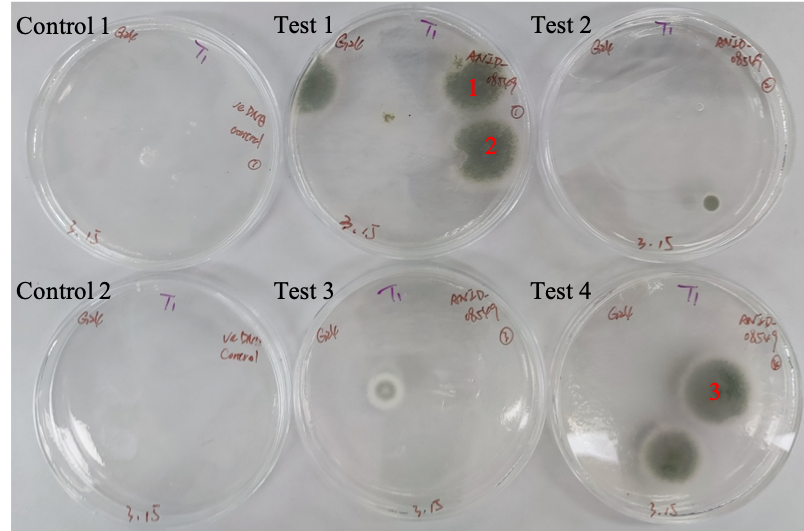
\includegraphics[width=0.45\textwidth]{6.png}
\captionsetup{font={scriptsize,bf,stretch=1}}
\caption{\scriptsize \textbf{Positive screening for mutant strains with selective agar plates in which regeneration media absent the uridine and uracil. Controls 1 and 2 were negative controls which inoculated with Aspergillus nidulans that were not transformed with ANID\_08549 DNA cassette. Test plates 1, 2, 3 and 4 were inoculated with the same volume of medium with the Aspergillus nidulans strain that was transformed with ANID\_08549 DNA cassette. The putative transformant colonies labelled 1, 2 and 3 in red were later amplified on agar plates. }}
\label{fig1}
\end{figure}


Figure\ref{fig2} illustrates the negative strain, Putative transformants 1 and 2 which were amplified on the agar plates. Both negative strain and transformants generated dark green colonies and white hyphae. The morphology of the transformants does not have a significant difference from the negative strain. The most noticeable variance might be the transformants generated more hyphae and the colonies’ colour was lighter compared to the negative strain. The strains on these three plates were later performed PCR to determine whether the transformants had successfully deleted the gene ANID\_08549 by homologous recombination and displaced the Af-pyrG gene to the genome.


According to the Data analysis sheet (Appendix 1), if the gene ANID\_08549 was not deleted by homologous recombination using the ANID\_08549 DNA cassette, such as the negative strain and the transformants which have the false positive results, the PCR products that were amplified by diagnostic primers ANID\_08549F and ANID\_08549R would have the length of 975 bp, while the transformants which have already deleted the gene ANDI\_08549 and replaced it with the Af-pyrG gene would not generate PCR product at the size of 975 bp. On the contrary, the PCR products of transformants which have already deleted the gene ANID\_08549 and replaced it with the Af-pyrG gene, which was amplified by diagnostic primers ANID-08549F and Af-Revers would at the size of 865 bp, whereas the negative strain and the transformants which have the false positive results would not generate PCR product at the size of 865 bp.


\begin{figure}[H]
\centering
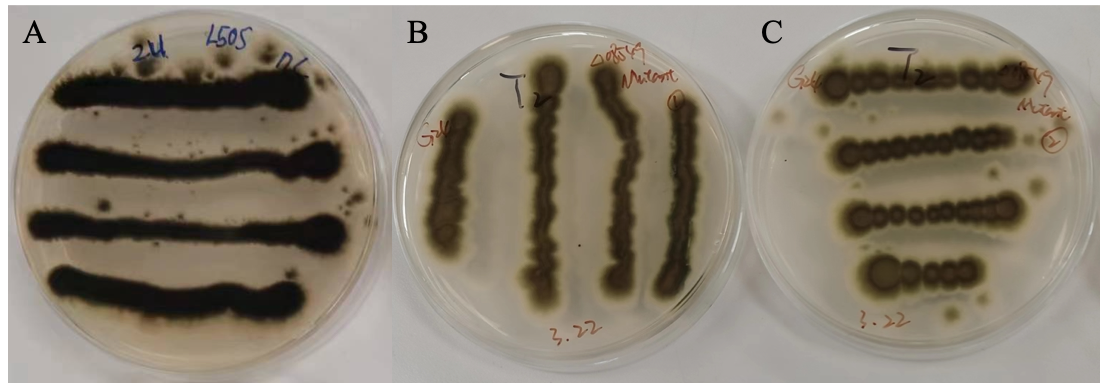
\includegraphics[width=0.45\textwidth]{3.png}
\captionsetup{font={scriptsize,bf,stretch=1}}
\caption{\scriptsize \textbf{Amplification of putative transformants and negative strain. Negative strain (A), transformants 1 (B) and transformant 2 (C).}}
\label{fig2}
\end{figure}


\begin{figure*}
\centering
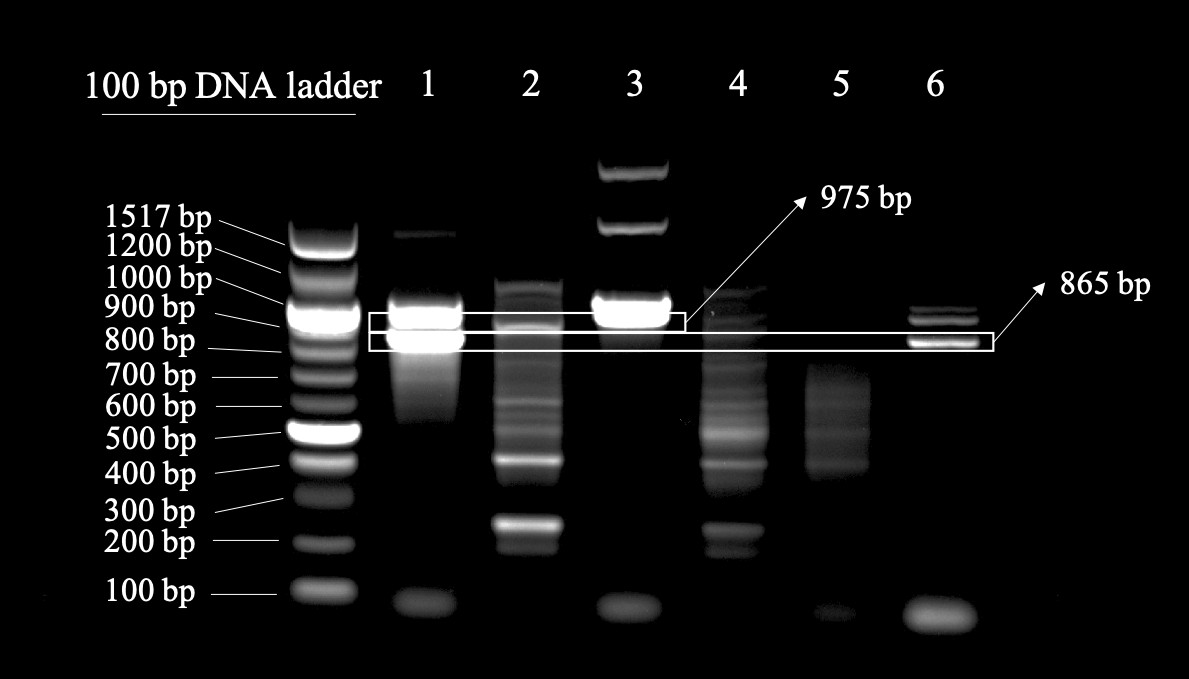
\includegraphics[width=0.95\textwidth]{gel.jpg}
\captionsetup{font={scriptsize,bf,stretch=1}}
\caption{\scriptsize \textbf{PCR verification for putative transformants 1 and 2. Lanes 1 and 2 were set as negative controls which added the genome of the negative strain as a template. Lanes 3 and 4 added the genome of transformant 1 as a template. Lanes 5 and 6 added the genome of transformant 2 as a template. Samples of lanes 1, 3 and 5 were amplified DNA with diagnostic primers ANID\_08549F and ANID\_08549R. Samples of lanes 2, 4 and 6 were amplified DNA with diagnostic primers ANID\_08549F and Af-Revers. }}
\label{fig3}
\end{figure*}


As Figure\ref{fig3} illustrates, lane 1 generated a wide, bright band at around 900-1000 bp which meets the expectation that the negative strain possessing the gene ANID\_08549 would have PCR products with the size of 975 bp. However, a band which has a size of around 800 bp is shown unexpectedly at lane 1. The reasonable explanation for this phenomenon is that the negative strain sample has been contaminated by the other strains during the DNA extraction. The spatula which was used for the sample taking might not have been fully sterilized.


As for lanes 3 and 4, the genomes added were extracted from putative transformants 1. Lane 3 generated a bright band with a size of around 975 bp while Lane 4 only generated multiple weak bands which indicates that transformant 1 is a false-positive strain which could result from the non-homologous end join (NHEJ). The cassette might be integrated into the genome other than the gene ANID\_08549 locus due to the NHEJ. When fungi genomes undergo double-strand breaks (DSBs), the genome is mainly repaired by non-homologous end joining or homologous recombination (HR)\cite{li2019pathways}. A linear DNA fragment is known to be able to be integrated into the fungal genome by NHEJ and this phenomenon has already been applied in a plasmid construction technique called gap repair cloning (GRC) on fungi\cite{corrigan2013fate}. The deletion cassette constructed in this experiment is a linear DNA fragment that could be integrated into the A. nidulans’ genome by NHEJ if there happen to be DSBs on the genome. The cassette integrated into the genome by NHEJ is not specific in other words the location of the integration is unknown. The PCR verification using the diagnostic primers ANID\_08549F and ANID\_08549R can still generate DNA fragments which have the size of 975 bp due to the gene  not having been deleted by the cassette. However, DNA verification by diagnostic primers ANID\_08549F and Af-Revers could not generate any DNA fragment with the size of 865 bp due to the primer ANID\_08549F being specifically combined with the sequence which is located upstream of the upstream homologous arm. (Appendix 1) The false positive could also be caused by the spontaneous mutation of the wild-type strains and the mixture of the transformant and the wild strain.


\iffalse
\begin{center}
{\footnotesize Table 4. Statistics on the number of colonies in groups 8 and 23}
\vspace{0pt}
\begin{table}[H]
\setlength{\tabcolsep}{5pt}
\footnotesize
\begin{tabular}{ccccccccccccc}
\toprule [1pt]
Plates&1&2&3&4&5&6&7&8&9&10&11&12\\
\hline
G8&/&1&3&5&550&56&44&91&6&6&21&6\\
G23&/&2&12&3&680&142&48&70&2&5&3&48\\
\bottomrule [1pt]
\end{tabular}
\end{table}
\end{center}
\fi


For lanes 5 and 6, there are no significant bands with a size of around 975 bp at lane 5 and lane 6 possesses a band that has a size of around 865 bp which indicate that the putative transformant 2 is verified to be a transformant. There are multiple bands shown in lanes 2, 4 and 5 which could be due to the low specificity of the diagnostic primers and the primers might bind on multiple sites on the genome.


According to Appendix 1, the gene ANID\_08549 has the Lamin A/C globular tail domain which belongs to the Lamin tail domain superfamily. The Lamin tail domain which could be found as Nuclear Lamins has an immunoglobulin (Ig) fold structure\cite{dittmer2011lamin}. The expression product of gene ANID\_08549 might have the ability to mediation diverse protein-protein and protein-ligand interactions by the possession of Lamin A/C globular tail domain.


\section{Discussion and Conclusion}


Observing the gel electrophoresis results of all the experimental groups involving the ANID\_08549 gene, it is evident that a large number of non-specific bands appear in multiple electrophoresis lanes of each experimental group. The cause of this phenomenon could be contamination of DNA impurities, insufficient primer specificity, among other factors. DNA contamination can occur at various stages, including DNA extraction and PCR substrate contamination, which can lead to the appearance of unknown DNA bands. Standardizing experimental procedures, using a laminar flow hood, and flame sterilization to prevent microbial contamination can help minimize DNA sample contamination. The design of primers is crucial for the success of the experiment. When designing primers, attention should be paid to the CG content of the primers to ensure the Tm value is within a reasonable range. The primer sequence should not complement itself to avoid self-folding into a hairpin structure\cite{singh2000effect}. Additionally, the primers should not have high binding affinity to other positions on the DNA template, ensuring that the PCR results targeting specific fragments are more accurate. The three primers, ANID\_08549F, ANID\_08549R, and Af-Rev, have Tm values of 58, 56, and 49 degrees Celsius, respectively. The CG content of the Af-Rev primer is only 38\%, while the optimal GC content for primers is between 50\% and 60\%, and the Tm value should be between 55 and 60 degrees Celsius. Improvements should be made to the Af-Rev primer in future experiments. \hyperref[secB]{AppendixB} is the results of primer-specific analysis of the entire genome of Aspergillus nidulans using Primer-blast, it is found that the ANID\_08549F and ANID\_08549R primers do not exhibit strong specificity within the entire genome. Apart from the expected 975 bp DNA product, multiple DNA subchains such as 942, 790, and 525 bp are also produced, consistent with the gel electrophoresis results. Moreover, there is a probability of self-complementarity in the primers, which can affect the PCR results. Therefore, there are significant flaws in the PCR primer design of this experiment, and in future experiments, primers with higher specificity should be designed to ensure clearer and more accurate experimental results.


Reverse genetics methods allow researchers to determine the function of a gene by detecting changes in the gene's phenotype, which in this experiment could not be known simply by observing changes in appearance.Experimental results indicate that ANID\_08549 has been successfully replaced by Af-pyrG, so it is necessary to predict the function of ANID\_08549 and then determine how this gene affects biological processes. By comparing the results of biological processes in the experimental group and the control group, it can be determined whether the molecular function is consistent with expectations, and thus the function of the gene can be determined. ANID\_08549 is annotated as a gene encoding a protein of unknown function based on gene structure analysis \hyperref[secC]{(AppendixC)}\cite{wortman20092008}. The hypothetical protein is 394 amino acids long. The InterPro analysis of the protein structure reveals that amino acids 1-239 constitute a DUF2278 domain, and amino acids 302-370 constitute a Lamin A/C globular tail domain\hyperref[secD]{(AppendixD)}\cite{paysan2023interpro}. The function of the DUF2278 domain is unknown, while the Lamin A/C globular tail domain is known to mediate protein-protein interactions. However, the protein function cannot be determined through domain analysis alone. Further sequence comparisons using BLAST reveal multiple proteins with known functions that are identical to ANID\_08549. These proteins are all O-methyltransferases. Analyzing these proteins can help further determine the function of the ANID\_08549 protein. By comparing multiple sequences, it is observed that the similarity between the two protein sequences is high, and there are many same motifs scattered throughout the entire sequence \hyperref[secF]{(AppendixF)}. Structural domain analysis of the O-methyltransferase reveals that this protein also possesses DUF2278 and Lamin A/C globular tail domains\hyperref[secE]{(AppendixE)}, and has a similar length. Based on the above analysis, it is hypothesized that ANID\_08549 encodes a protein that is an O-methyltransferase.

Further determine the target of the protein modification to clarify the specific role of the gene. Methyltransferases typically catalyze the transfer of a methyl group from S-adenosyl-L-methionine (AdoMet) to a nucleophilic center on the target substrate\cite{ferrer2005crystal}, which can be C, O, N, or S-centered. O-methyltransferases, in particular, transfer a methyl group from the donor molecule to the oxygen atom of the acceptor molecule. Methyltransferases can modify proteins, DNA, RNA, or other small molecules. Most O-methyltransferases discovered so far are involved in modifying small molecules, such as Caffeoyl-CoA O-methyltransferase and Catechol-O-methyltransferase\cite{vidgren1994crystal}.In future work, it will be important to determine the specific target of this O-methyltransferase. Metabolomics analysis of the experimental and control fungal groups can be conducted using gas chromatography-mass spectrometry (GC-MS) and other methods\cite{david2008analysis}\cite{albright2015large}. By comparing the types of small molecule metabolites, we can determine the targets of methylation by the methyltransferase, further elucidating the impact of this gene on cellular metabolic pathways and accurately determining the gene's function.


This experiment represents the first step in reverse genetics to validate gene function by knocking out and replacing the gene under study. The results indicate that the ANID\_08549 positive experimental strain was successfully replaced by the Af-pyrG gene, and the replaced strain was able to survive on agar plates lacking uracil and uridine. However, the replacement results are still unstable, and the appearance of false positives and unknown DNA bands has added more uncertainty to the experiment. It is necessary to repeat the experiment to verify the randomness of false positives and to optimize the PCR primers to obtain better gel electrophoresis results and a stronger confirmation that the ANID\_08549 gene has been successfully replaced. Through bioinformatics analysis, it was determined that the protein encoded by the ANID\_08549 gene is an O-methyltransferase. In future work, a series of biochemical methods and metabolomics approaches will be used to determine the interaction between this protein and small molecules, further elucidating the function of the ANID\_08549 gene.


~\\
~\\
\bibliographystyle{unsrt}
\bibliography{reference}

\end{multicols}


\clearpage


\begin{appendices}
\section*{Appendix A. Data Analysis Sheet}\label{secA}

\textbf{Authors:} Mingbai.Zeng, Kangyao.Ma, Haozhan.Yuan, Yimeng.Yuan\\
\textbf{Date:} 2024.4.12\\
\textbf{Gene Name:} Uncharacterized\\
\textbf{Systemic Name:} AN8549, ANID\_08549\\
\textbf{Description:} Uncharacterized protein\\
\textbf{References:}For A. nidulans – none available\\
\textbf{GO annotation:}\\
GO:0008150 Biological Process\\
GO:0005575 Cellular Component\\
GO:0003674 Molecular Function\\
\textbf{S. cerevisiae Homologue:}\\
\textbf{Protein Sequence:}\\
\textgreater AN8549-T $\mid$ Aspergillus nidulans FGSC A4 $\mid$ segment length=394\\
\texttt{MPVDNYGVLKCRAITYKLEDGQQSPRAPQLSLYVRDTGSPTSQLNGHLQEARAGLPVHRAAINITSGDLDDSR\\
LAYWVNHQIGQNPIVNRLSQLEYGFHPVENNKTLGLDYIRDSLFTSTNGRLLPHDIPGQYTDIIDVLSPYIQH\\
AVREKANLYLFGSESRSDTRGSAPVIHNIHMNQGNARKFRADDGVFQDGGLIFHFPCARPDSDTGCVEDRPRG\\
EWLGIFLAFASQAVHTNPSSGHAISGVGWSDILRPDIIEEGVVIREARLHLDSSGTDADAVTDESETGARPCI\\
GRRKSISLTVTLSNHTNRAVRLGDWTIRNRSGCVHTLPRGIALRPMVDQHFELGDYTLSEDGDTILLLNEHGL\\
KVDGVSYNSAQEGMGLKGKGKGGSIVFVH}\\
\textbf{Pfam domains:}\\
1 Lamin tail domain superfamily, Lamin A/C globular tail domain\\
\textbf{Primers used for Deletion cassette:}\\
5 forward: \texttt{GTAACGCCAGGGTTTTCCCAGTCACGACGGAGACTCATACAGCCCTACC}\\
5 Reverse: \texttt{ATCCACTTAACGTTACTGAAATCTCAAGACCCCGTAGTTGTC}\\
3 forward: \texttt{CTCCTTCAATATCATCTTCTGTCGAGAGAAAAGGAGTGAGGTG}\\
3 Reverse: \texttt{GCGGATAACAATTTCACACAGGAAACAGCAAGCAGACAGTAACCCTAGC}\\
\textbf{Diagnostic primers and expected product size for wild type:}\\
ANID\_08549F: \texttt{TCGCAGGTCCCAGTGATG}\\
ANID\_08549R: \texttt{GTCCATCCCAGCCATTTG}\\
PCR product size in the wild type: 975 bp\\
\textbf{Diagnostic primers and expected product size for mutant:}\\
ANID\_08549F: \texttt{TCGCAGGTCCCAGTGATG}\\
Af-Rev: \texttt{CCACTTAACGTTACTGAAATC}\\
PCR product size in the mutant: 865 bp\\
\textbf{Annotated DNA sequence:}\\
(Note: The sequence in red indicates the intron of the genome, and the sequence in blue indicates the open reading frame (ORF) of the gene ANID\_08549 and PyrG gene. The sequences that are highlighted are the primers used in the lab session)
\begin{figure}[H]
\centering
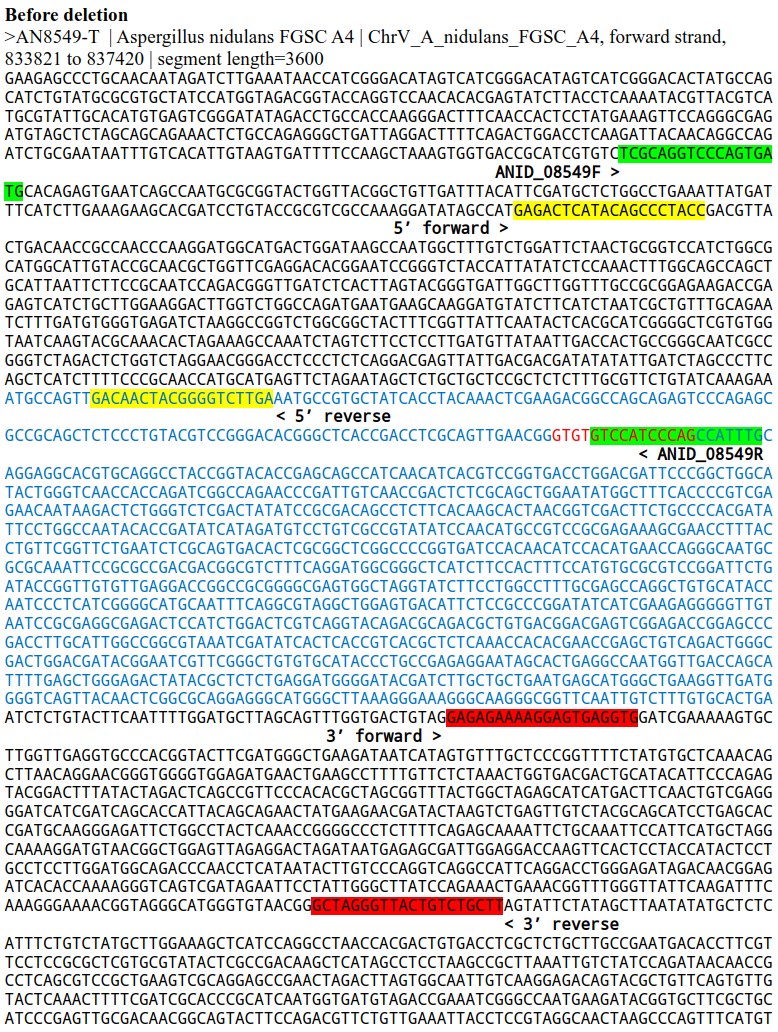
\includegraphics[width=0.95\textwidth]{before.png}
%\captionsetup{font={scriptsize,bf,stretch=1}}
%\caption{\scriptsize \textbf{Amplification of putative transformants and negative strain. Negative strain (A), transformants 1 (B) and transformant 2 (C).}}
%\label{fig4}
\end{figure}

\begin{figure}[H]
\centering
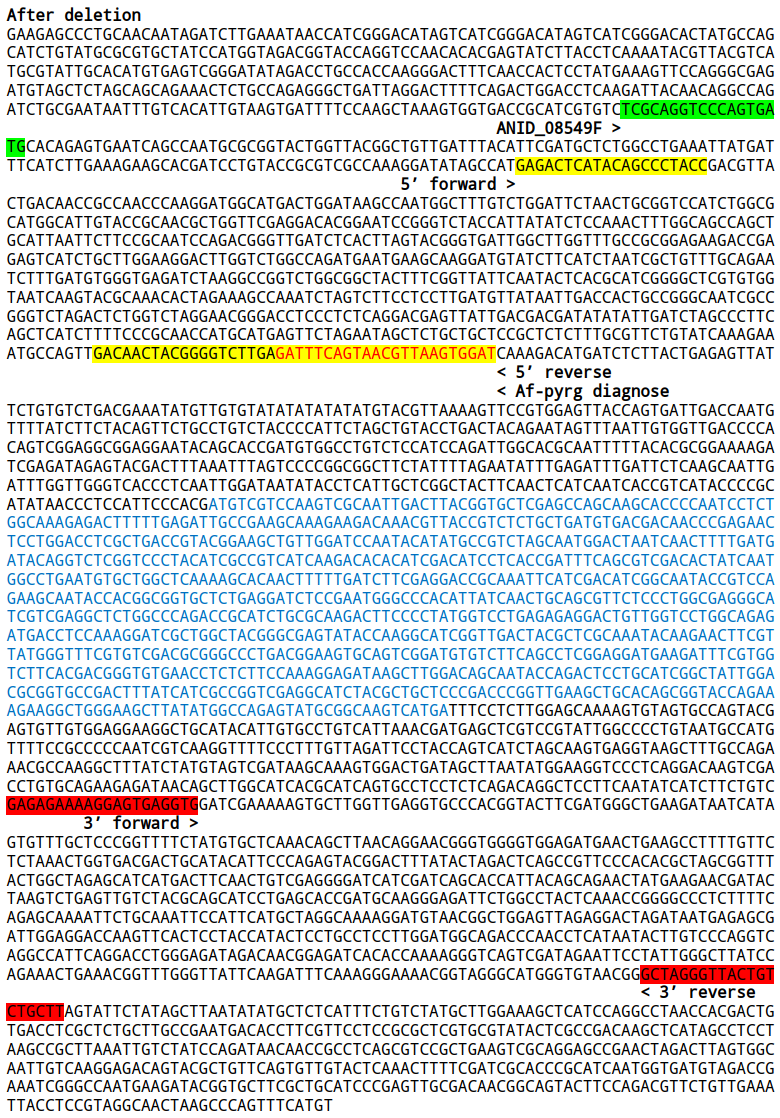
\includegraphics[width=0.95\textwidth]{after.png}
%\captionsetup{font={scriptsize,bf,stretch=1}}
%\caption{\scriptsize \textbf{Amplification of putative transformants and negative strain. Negative strain (A), transformants 1 (B) and transformant 2 (C).}}
%\label{fig4}
\end{figure}


\section*{Appendix B. Prediction of molecular structure of hypothetical protein AN8549}\label{secB}

\begin{figure}[H]
\centering
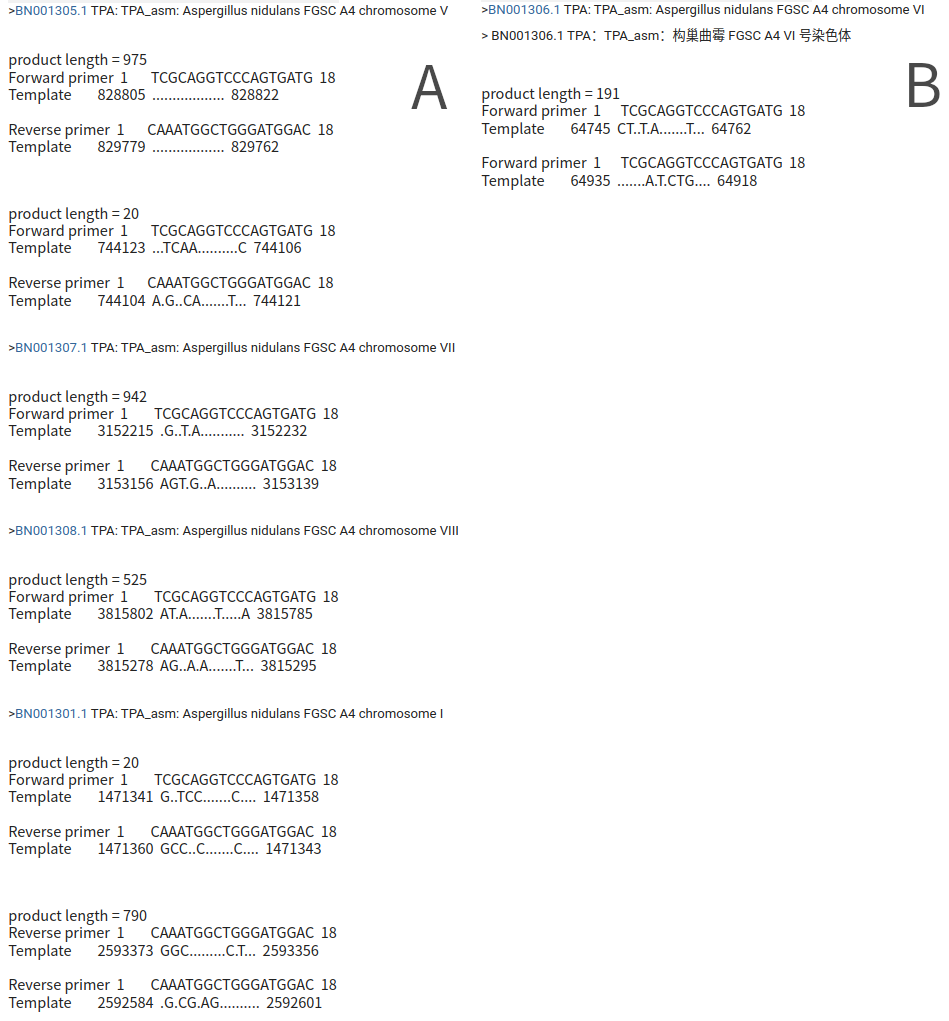
\includegraphics[width=0.95\textwidth]{primerblast.png}
%\captionsetup{font={scriptsize,bf,stretch=1}}
%\caption{\scriptsize \textbf{Amplification of putative transformants and negative strain. Negative strain (A), transformants 1 (B) and transformant 2 (C).}}
%\label{fig9}
\end{figure}


~\\
~\\
~\\
~\\
\section*{Appendix C. Location of AN8549 gene in Aspergillus nidulans}\label{secC}

\begin{figure}[H]
\centering
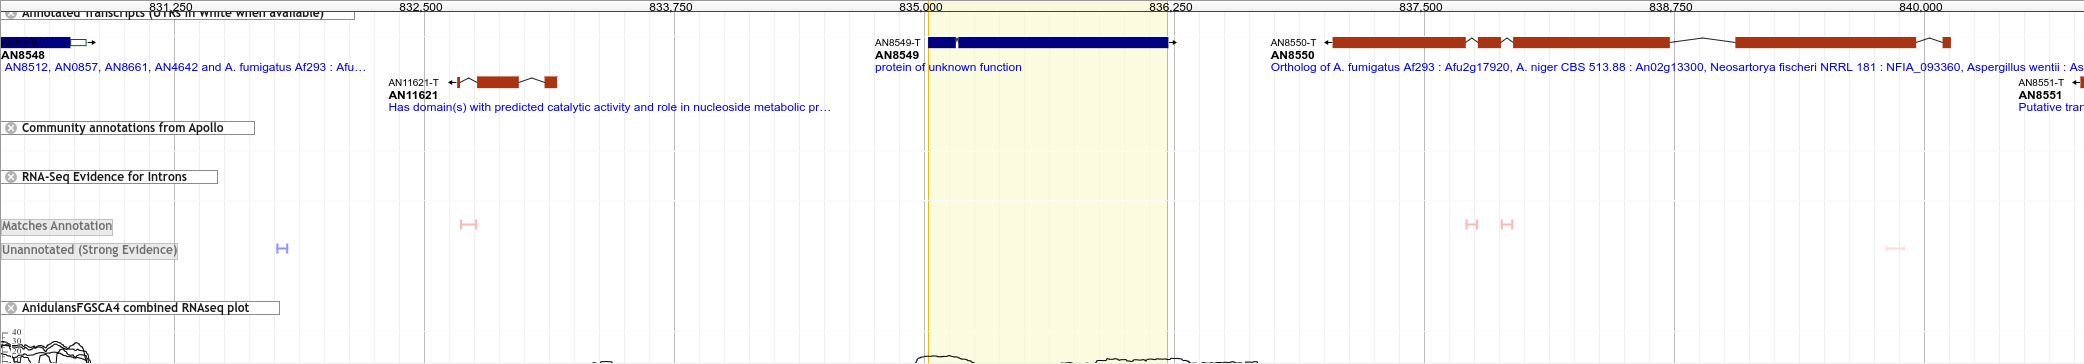
\includegraphics[width=0.95\textwidth]{AN08549.png}
%\captionsetup{font={scriptsize,bf,stretch=1}}
%\caption{\scriptsize \textbf{Amplification of putative transformants and negative strain. Negative strain (A), transformants 1 (B) and transformant 2 (C).}}
%\label{fig4}
\end{figure}
~\\
~\\

\section*{Appendix D. Prediction of domain structure of hypothetical protein AN8549\cite{paysan2023interpro}}\label{secD}

\begin{figure}[H]
\centering
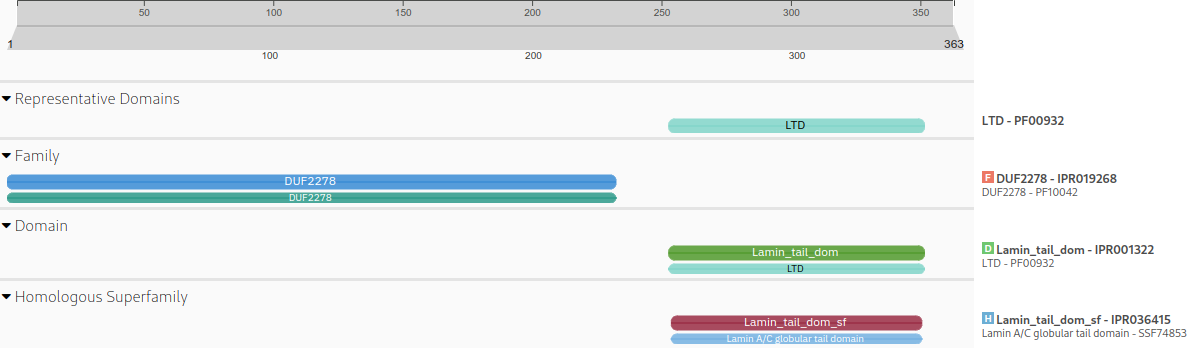
\includegraphics[width=0.95\textwidth]{BO83DRAFT_454721domain.png}
%\captionsetup{font={scriptsize,bf,stretch=1}}
%\caption{\scriptsize \textbf{Amplification of putative transformants and negative strain. Negative strain (A), transformants 1 (B) and transformant 2 (C).}}
%\label{fig5}
\end{figure}
~\\
~\\

\section*{Appendix E. Prediction of O-methyltransferases domain of AN8549 homologous protein\cite{paysan2023interpro}}\label{secE}

\begin{figure}[H]
\centering
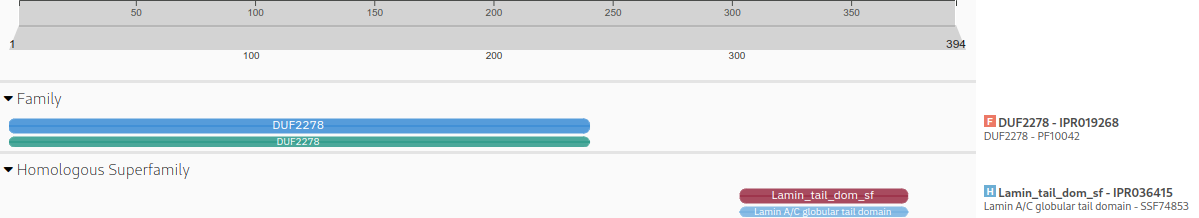
\includegraphics[width=0.95\textwidth]{8549domain.png}
%\captionsetup{font={scriptsize,bf,stretch=1}}
%\caption{\scriptsize \textbf{Amplification of putative transformants and negative strain. Negative strain (A), transformants 1 (B) and transformant 2 (C).}}
%\label{fig6}
\end{figure}


\section*{Appendix F. Sequence comparison results of hypothetical protein AN8549 and O-methyltransferases}\label{secF}

\begin{figure}[H]
\centering
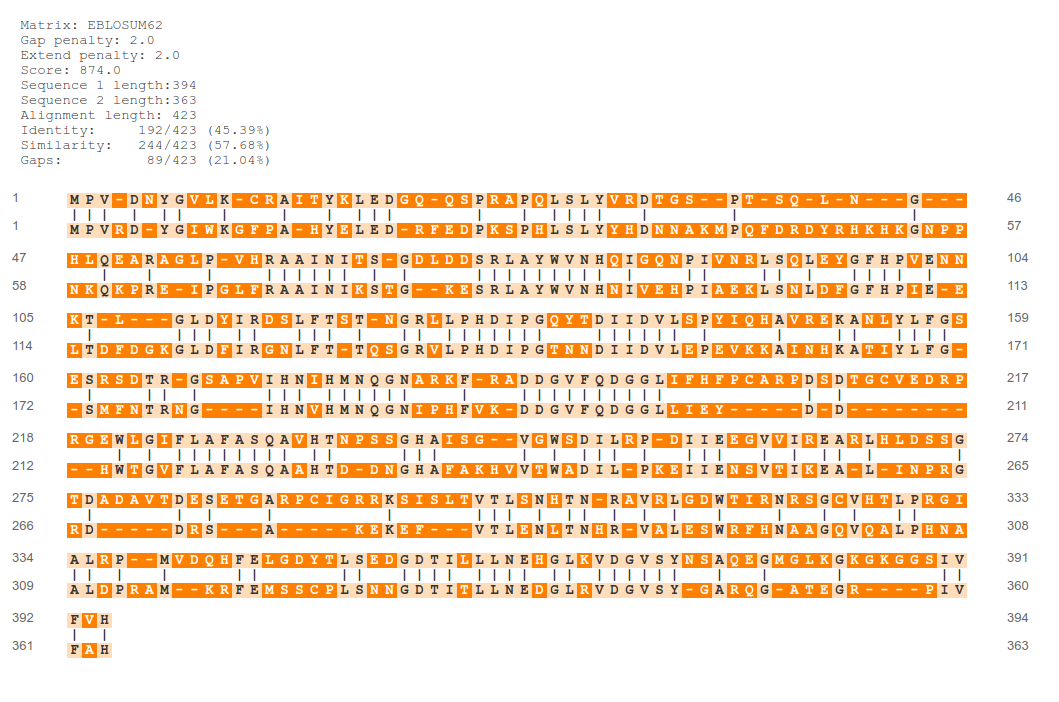
\includegraphics[width=0.9\textwidth]{two.png}
%\captionsetup{font={scriptsize,bf,stretch=1}}
%\caption{\scriptsize \textbf{Amplification of putative transformants and negative strain. Negative strain (A), transformants 1 (B) and transformant 2 (C).}}
%\label{fig7}
\end{figure}


\section*{Appendix G. Prediction of molecular structure of hypothetical protein AN8549\cite{jumper2021highly}\cite{varadi2022alphafold}}\label{secG}

\begin{figure}[H]
\centering
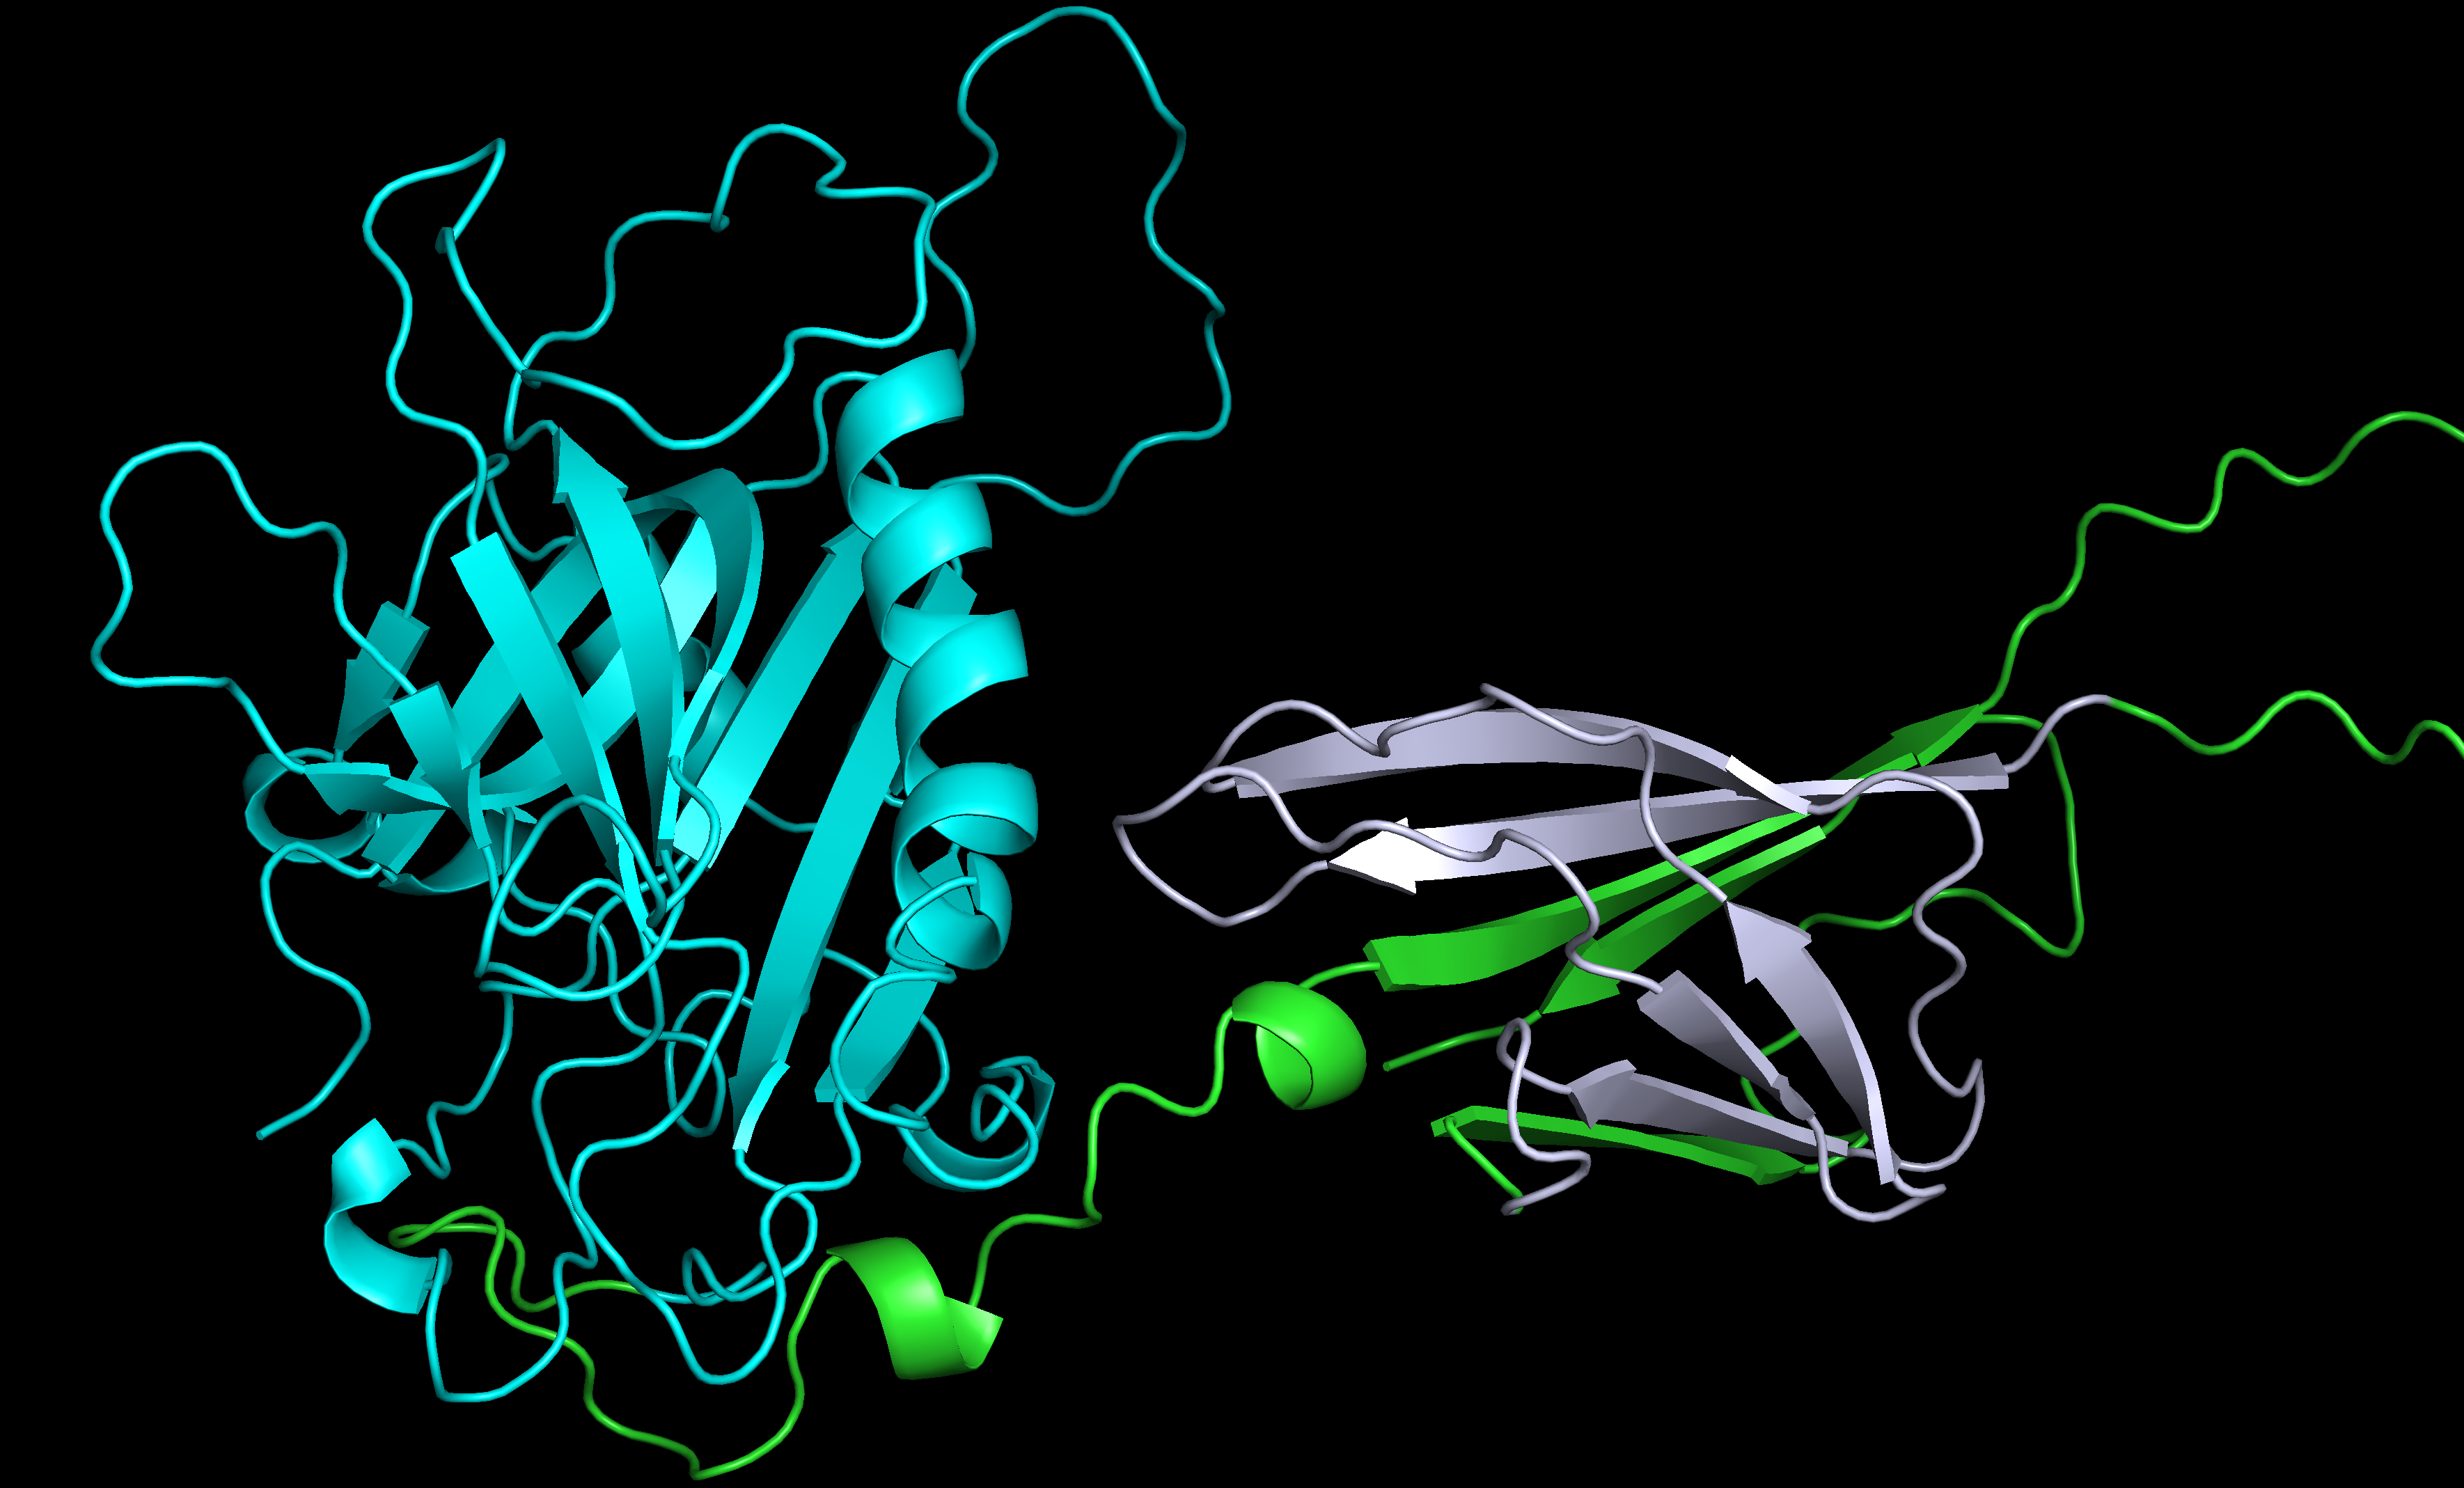
\includegraphics[width=0.9\textwidth]{twodomain.png}
%\captionsetup{font={scriptsize,bf,stretch=1}}
%\caption{\scriptsize \textbf{Amplification of putative transformants and negative strain. Negative strain (A), transformants 1 (B) and transformant 2 (C).}}
%\label{fig8}
\end{figure}



\end{appendices}


\includepdfmerge{question1.pdf}

\end{document}
